\documentclass[conference]{IEEEtran}

\usepackage{cite}
\usepackage{amsmath}
\usepackage{graphicx}
\usepackage{booktabs}
\usepackage{array}

\begin{document}

\title{Comparing Text Representations and Classifiers for Twitter Sentiment Analysis}

\author{
\IEEEauthorblockN{Author One}
\IEEEauthorblockA{Student ID: 00000000\\
MSc in Applied Artificial Intelligence\\
South East Technological University\\
Ireland}
\and
\IEEEauthorblockN{Author Two}
\IEEEauthorblockA{Student ID: 00000000\\
MSc in Applied Artificial Intelligence\\
South East Technological University\\
Ireland}
}

\maketitle

\begin{abstract}
This paper compares the text representations and classifiers required for binary Twitter sentiment analysis. The same held-out test set is used throughout. Bag-of-words, term frequency, inverse document frequency, and TF--IDF are compared under a fixed logistic regression classifier, then TF--IDF is held fixed while Naive Bayes, L1 and L2 logistic regression, and a ReLU network are compared. A sentence convolutional network is then used to test word order, dropout, batch normalisation, and transfer from pretrained GloVe vectors. On 1{,}998 test tweets, inverse document frequency with L2 logistic regression reaches a macro F1 of 0.806. The four sparse weightings differ by only 0.007. Mean-pooled embeddings fall to 0.746 because they discard local word order. Removing stopwords lowers macro F1 by 0.043 because negation is removed with them. Magnitude pruning shows that most fitted neural weights are unused.
\end{abstract}

\begin{IEEEkeywords}
sentiment analysis, TF--IDF, word embeddings, convolutional neural networks, regularisation
\end{IEEEkeywords}

\section{Introduction and Motivation}
Short social-media text is a hard sentiment task because the label often depends on a short phrase rather than on a single word. A count of \emph{bad} is not the same evidence as the phrase \emph{not bad}, and a tweet can contain both a compliment and a complaint. The practical question is which part of the pipeline changes the decision: the cleaning, the numeric representation, or the classifier.

This study answers that question with controlled comparisons. Each experiment changes one factor and reports accuracy and macro F1 on tweets that were not used to choose any setting. The representations are bag-of-words, term frequency (TF), inverse document frequency (IDF) \cite{sparckjones1972idf}, TF--IDF \cite{salton1988term}, Word2Vec \cite{mikolov2013word2vec}, and pretrained GloVe \cite{pennington2014glove}. The classifiers are multinomial Naive Bayes \cite{mccallum1998nb}, L1 and L2 logistic regression, a one-hidden-layer network with ReLU and dropout \cite{srivastava2014dropout}, and a sentence convolutional network \cite{kim2014cnn} with batch normalisation \cite{ioffe2015batchnorm}.

\section{Experimental Setup}
The corpus is the supplied Twitter collection. Each line is one tweet and the filename is the label. The training pool contains 399{,}000 positive and 399{,}000 negative tweets. A stratified sample of 50{,}000 tweets from each class was drawn with seed 42. Ten percent of that sample, 10{,}000 tweets, was used only to choose hyperparameters. Every reported score uses the full test files: 1{,}000 positive and 998 negative tweets.

After the final cleaning, tweets average 13.0 tokens in both the sample and the test set. Positive and negative tweets have nearly the same length, so a later gap is not caused by one class being longer. Cleaning leaves 206 empty training tweets and 6 empty test tweets, usually because the original text was only a URL or a mention. Empty tweets become zero vectors.

The sparse vectoriser uses unigrams and bigrams, a minimum document frequency of 2, and at most 20{,}000 features. Logistic regression uses the liblinear solver. The regularisation strength $C$ is chosen from $\{0.01, 0.1, 1, 4, 10\}$ on the validation split for the TF--IDF algorithm study, and from $\{0.1, 1, 4\}$ for the other representations. Neural models use Adam with learning rate $10^{-3}$ and L2 weight decay $10^{-4}$. The convolutional network pads every tweet to 40 tokens.

\section{Methodology}
Preprocessing is separated from vectorisation. Preprocessing only cleans the string. Vectorisation then turns that string into numbers. The cleaning used in every later experiment lowercases the text, removes URLs and @mentions, expands contractions so that \emph{n't} remains \emph{not}, and deletes digits and punctuation. Stopwords are kept. To test that choice, TF--IDF and L2 logistic regression are held fixed at $C=1$ and only the cleaning is changed.

The representation study then holds the classifier fixed as L2 logistic regression. Bag-of-words stores raw n-gram counts. TF replaces those counts by an L2-normalised frequency and disables IDF. IDF records each n-gram as present or absent and multiplies it by a smoothed inverse document frequency, which isolates rarity from repetition inside one short tweet. TF--IDF uses sublinear term frequency times the same IDF weight. Word2Vec is a 100-dimensional skip-gram model trained only on the training text; a tweet is the mean of its in-vocabulary word vectors. GloVe uses the pretrained 100-dimensional Twitter table in the same way, so it is the transfer-learning case of a mean embedding.

The algorithm study freezes the representation at TF--IDF. Multinomial Naive Bayes is tuned by its smoothing value $\alpha \in \{0.1, 0.5, 1.0\}$. L1 and L2 logistic regression are tuned by $C$. The artificial neural network has one hidden layer, a ReLU activation, dropout, and L2 weight decay. Hidden size is chosen from $\{64, 128\}$ and dropout from $\{0.0, 0.2, 0.5\}$.

The convolutional network reads the tweet as a sequence, so it can respond to a local pattern such as \emph{not bad} \cite{kim2014cnn}. Filters of width 3, 4, and 5 are followed by ReLU and max-pooling. Dropout is selected on a network whose embeddings are trained from scratch. That rate is then fixed for four test models: scratch embeddings, the same model with batch normalisation, frozen GloVe embeddings, and GloVe embeddings that are fine-tuned. Batch normalisation and transfer are placed in separate rows so that each change has its own result.

Pruning is applied after training, with no retraining. L1 logistic regression is the feature-pruning result. Magnitude pruning then deletes the smallest weights of the trained network at 20\%, 50\%, and 80\%.

\section{Results and Discussion}
Figure~\ref{fig:prep} shows the preprocessing result. Macro F1 stays between 0.799 and 0.801 from lowercase-only text through the full cleaning. Deleting stopwords lowers it from 0.801 to 0.759. The useful cleaning step is therefore not URL removal. It is the decision to retain negation words.

\begin{figure}[t]
\centering
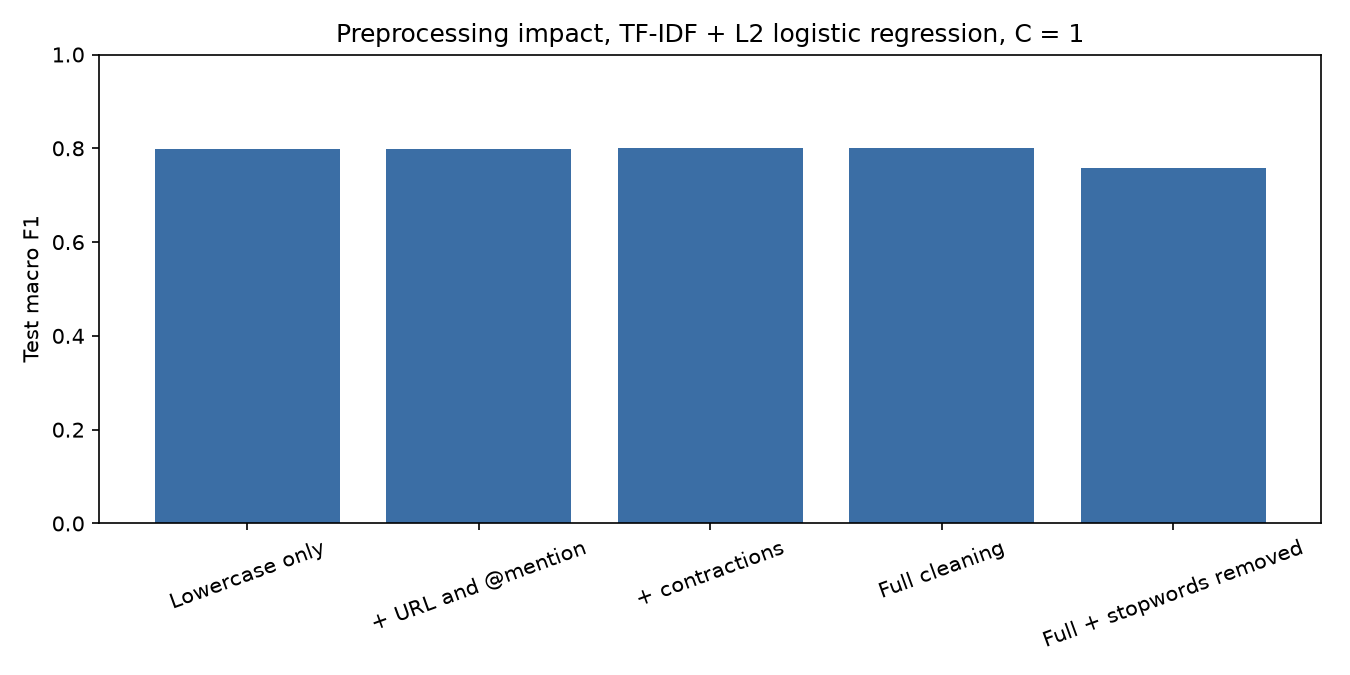
\includegraphics[width=\linewidth]{figures/preprocessing_impact.png}
\caption{Test macro F1 when only the cleaning changes. The classifier is TF--IDF with L2 logistic regression at $C=1$.}
\label{fig:prep}
\end{figure}

Table~\ref{tab:results} and Fig.~\ref{fig:models} collect the test scores. Among bag-of-words, TF, IDF, and TF--IDF, the largest gap is 0.007 macro F1. On a test set of 1{,}998 tweets, a binomial standard error near 0.80 accuracy is about 0.009, so that gap is inside sampling noise. IDF is numerically highest, at 0.806 accuracy and 0.806 macro F1, with positive and negative F1 of 0.806 and 0.805. Repeating a word inside one tweet adds little once bigrams are present. Both mean embeddings score 0.746. Averaging \emph{not} with \emph{bad} removes the phrase that the bigram model can store as its own feature.

With TF--IDF fixed, L2 logistic regression scores 0.801 at $C=1$. L1 logistic regression scores 0.804 at the same $C$ while keeping 4{,}555 of 20{,}000 weights. Naive Bayes, with $\alpha=0.5$, scores 0.774. The ReLU network scores 0.801 at 128 hidden units and dropout 0.5. Its validation macro F1 only moves from 0.790 to 0.793 across the dropout grid, so the extra non-linearity does not beat a linear model on this representation.

The convolutional network selects dropout 0.2; validation macro F1 is 0.749 at dropout 0.0 and 0.2, and 0.739 at 0.5. Test macro F1 is 0.766 from scratch and 0.766 with batch normalisation. Frozen GloVe raises it to 0.793, and fine-tuning raises it to 0.800. Pretrained vectors help. Batch normalisation does not help on these short tweets, and neither convolutional model passes IDF. Transfer learning is useful here as an initialisation, not as a reason to replace the sparse classifier.

Magnitude pruning supports the same reading of model capacity. The neural network stays at about 0.80 macro F1 after 80\% of its weights are removed. The fine-tuned convolutional network stays near 0.80 through 50\% removal and falls to 0.780 at 80\%. L1 had already shown that most input features can be deleted without losing the decision.

\begin{table}[t]
\caption{Test-set performance. Macro F1 is the selection metric.}
\label{tab:results}
\centering
\footnotesize
\setlength{\tabcolsep}{3pt}
\begin{tabular}{@{}lcc@{}}
\toprule
Model & Accuracy & Macro F1 \\
\midrule
Bag-of-words & 0.799 & 0.799 \\
TF & 0.800 & 0.800 \\
IDF + L2 logistic regression & 0.806 & 0.806 \\
TF--IDF + L2 logistic regression & 0.801 & 0.801 \\
TF--IDF + L1 logistic regression & 0.804 & 0.804 \\
Multinomial Naive Bayes & 0.774 & 0.774 \\
ANN (ReLU, dropout 0.5) & 0.801 & 0.801 \\
Word2Vec mean & 0.746 & 0.746 \\
GloVe mean & 0.746 & 0.746 \\
CNN, scratch & 0.766 & 0.766 \\
CNN, batch normalisation & 0.766 & 0.766 \\
CNN, frozen GloVe & 0.793 & 0.793 \\
CNN, fine-tuned GloVe & 0.800 & 0.800 \\
\bottomrule
\end{tabular}
\end{table}

\begin{figure}[t]
\centering
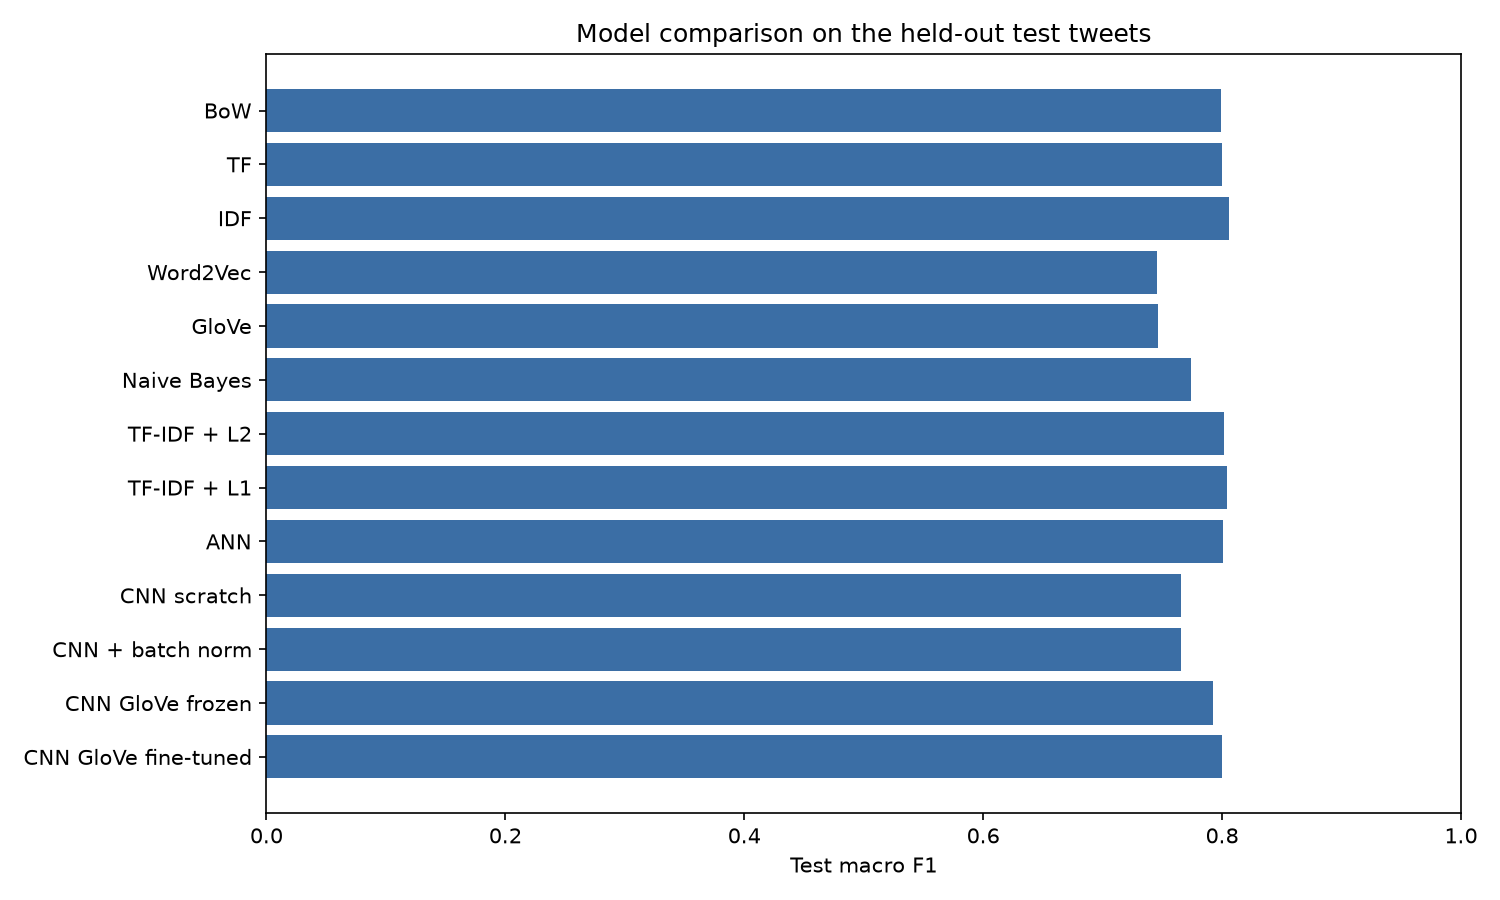
\includegraphics[width=\linewidth]{figures/model_comparison.png}
\caption{Test macro F1 for every final model. IDF with L2 logistic regression is the highest bar.}
\label{fig:models}
\end{figure}

\section{Error Analysis and Key Findings}
The overall score does not say which tweets fail. On the 487 test tweets that contain a negation word, TF reaches accuracy 0.797 and IDF reaches 0.791. Mean Word2Vec and mean GloVe fall to 0.717. The scratch convolutional network scores 0.737 on this slice, while the fine-tuned GloVe network scores 0.780. Word order helps only after the embedding already carries sentiment. It does not repair negation by itself.

High-confidence mistakes of the IDF model are mixed or weakly labelled rather than random. False positives include a college-day complaint with no clear negative word, an exhausted tweet that says ``can't wait'' and ``not feel'', a hangover remedy, a weekend tweet that pairs ``gorgeous'' with blisters, and a two-word reply. False negatives include a positive drinking idiom, a scheduling reply, ``summer is less than 24 hours away'', a tweet that opens with ``is not sleeping'' and then an insult, and a carnival tweet that pairs fatigue with pride. Several of these gold labels disagree with the visible sentence. That label noise is a ceiling on accuracy: the best model is already at 0.806, and the remaining errors are not solved by a larger network.

Three findings follow. First, for this collection, the representation family matters more than the weighting inside that family. Second, a linear model on n-grams is enough; dropout, batch normalisation, and a convolutional architecture do not raise the test score once transfer is removed. Third, pruning and L1 regularisation show that the fitted decision uses a small part of the available weights.

\section{Conclusion}
Binary sentiment on this Twitter sample is best predicted by an IDF-weighted bag of unigrams and bigrams with L2 logistic regression, at macro F1 0.806 on the untouched test files. TF--IDF, L1 logistic regression, and a small ReLU network are statistically tied with it. Mean-pooled Word2Vec and GloVe lose local phrases and cost about six points. A convolutional network becomes competitive only when it is initialised from GloVe, and it still does not pass the sparse model. The preprocessing result is equally specific: stopword removal harms the score because it deletes negation. Future work should keep the same test split and test whether a phrase-aware classifier can correct the mixed-sentiment errors without giving up the calibration of the linear IDF model.

\bibliographystyle{IEEEtran}
\bibliography{references}

\end{document}
